\begin{thebibliography}{9}

\bibitem{complexsystems}{
	A. Barrat, M. Barthélemy, A. Vespignani.
\newblock Dynamical Processes on Complex Networks.
\newblock \textit{Cambridge University Press}
\newblock Chapter 10, pp. 216-241

}

\bibitem{influentials}{
	D.J.Watts, P.S.Dodds.
\newblock Influentials, Networks, and Public Opinion Formation.
\newblock \textit{Journal of Consumer Research}
\newblock Vol 34, No. 4 (December 2007), pp. 441-458
}

\bibitem{word2mouth}{
	J.Goldenberg, B.Libai, Eitan Muller.
\newblock Talk of the Network: A Complex Systems Look at the Underlying Process of Word-of-Mouth.
\newblock \textit{Marketing Letters}
\newblock 12:3, 211-223, 2001
}
	


\end{thebibliography}






\section{Additional figures}

\begin{figure}
\begin{center}
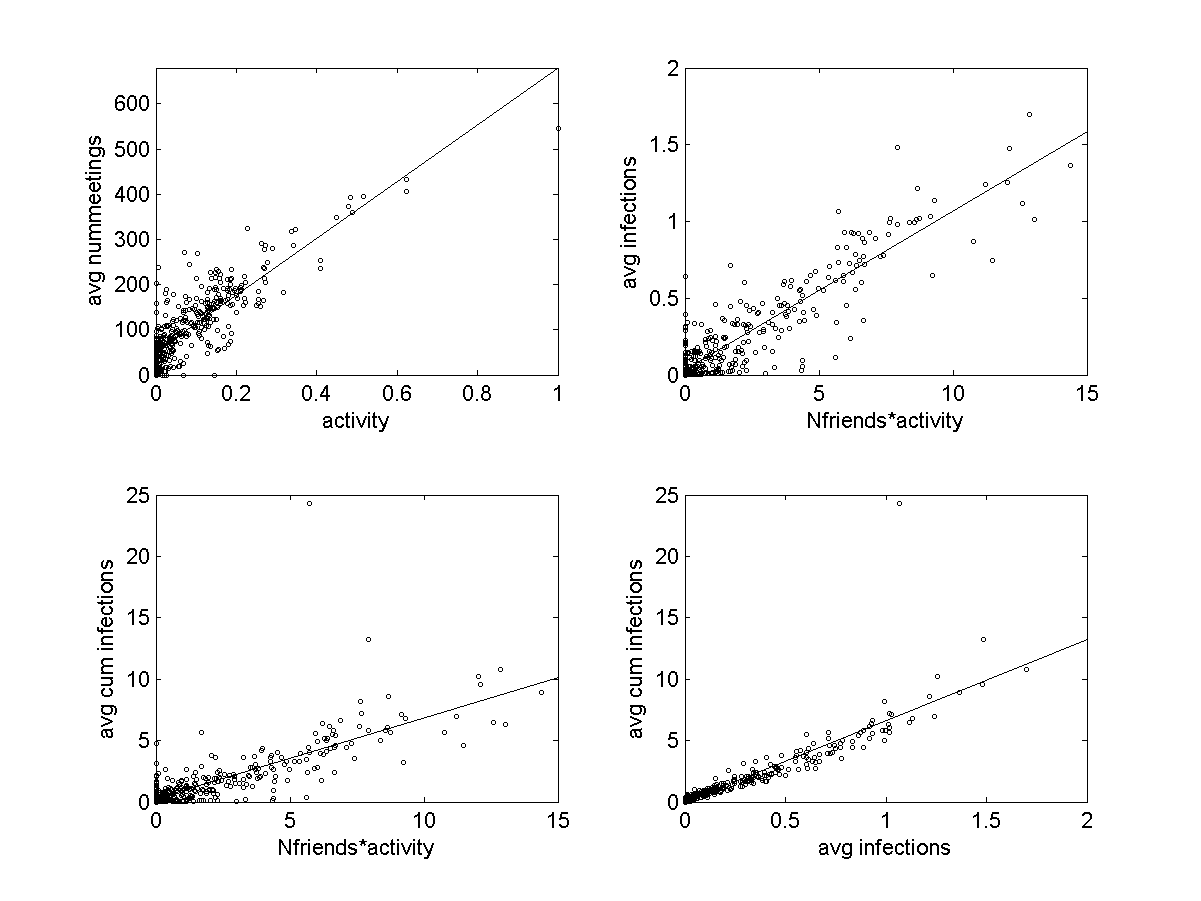
\includegraphics[width=16cm]{ImportantCorrelations}

\label{ImportantCorrelations}
\caption{Top left: Average number of meetings vs. activity. The trend line's slope is 630~$\frac{Avg.~nummeetings}{activity}$, R$^2$~=~0.71. Top right: Average number of infections vs. number of friends times activity. The trend line's slope is 0.10~$\frac{avg. infections}{Nfriends*activity}$, R$^2$~=~0.82. Bottom left: Average number of cumulative infections vs. number of friends times activity. The trend line's slope is 0.66~$\frac{Avg.~cum. infections}{Nfriends*activity}$, R$^2$~=~0.62. Bottom right: Average number of cumulative infections vs. number infections. The trend line's slope is  6.6~$\frac{avg.~cum.~infections}{avg.~infections}$ , R$^2$~=~0.82.}
\end{center}
\end{figure}

\begin{figure}
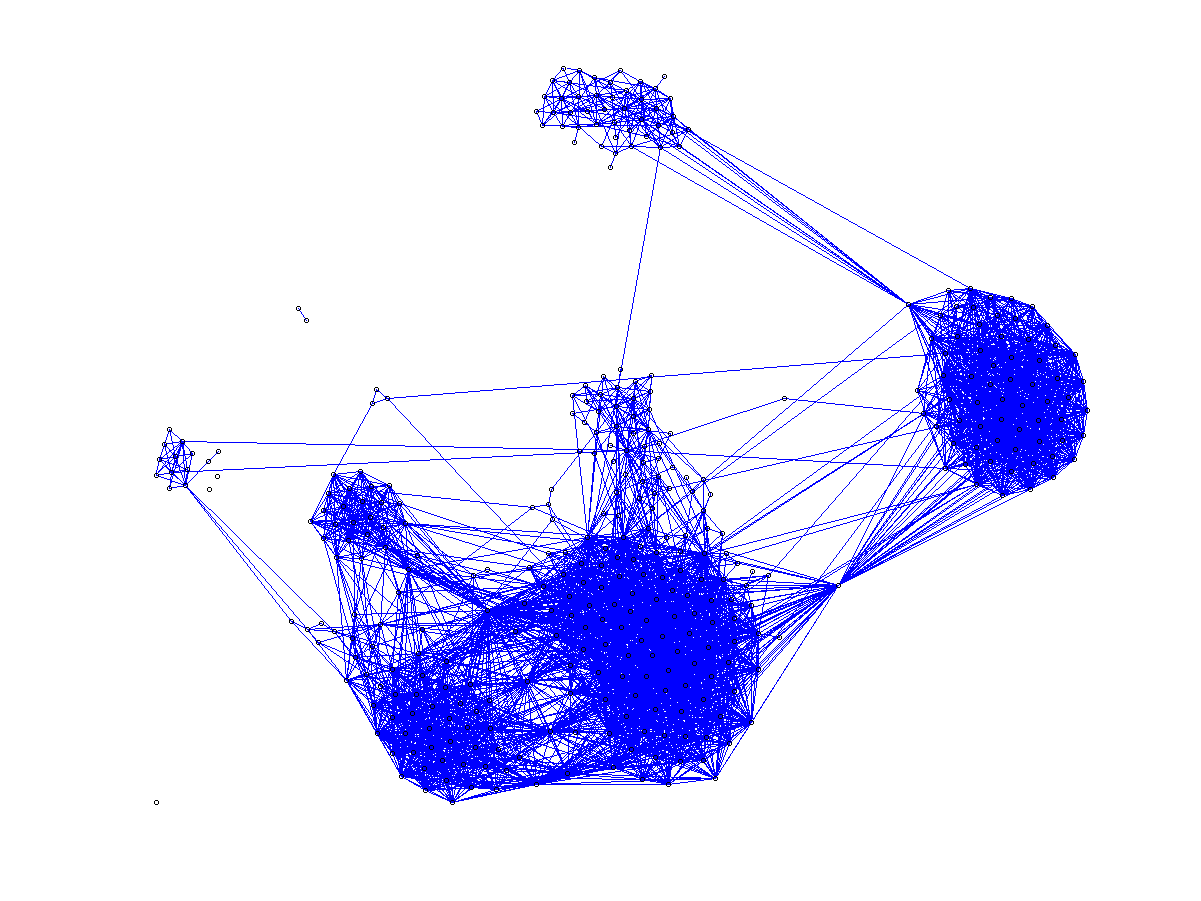
\includegraphics[width=7cm]{Network-Graph}
\caption{sdlhfa}
\label{Network-Graph}
\end{figure}